\section{Data}\label{data}

The dataset used in this shared task is the \ArgKP dataset~\cite{Bar-HaimEFKLS2020} which consists of 24\,083 argument and key point pairs labeled as matching/non-matching. They all belong to one of 28 controversial topics, for example: \textquote{Assisted suicide should be a criminal offence}. Each of the pairs is also assigned a stance towards the topic. 

The split used for training has 5\,583~arguments belonging to 207 key points within 24~topics. This leaves the 
validation dataset with 932~arguments and 36~key points for 4~topics. The test dataset, which is used for evaluation of all submissions, contains 723~ arguments with 33~ key points. There are 3~ topics given in the test dataset.

\subsection{Characteristics}
\begin{table*}
    \caption{Examples of \todo{matching} argument key point pairs from the \ArgKP dataset~\cite{Bar-HaimEFKLS2020}}
    \label{examples}
    \begin{tabularx}{\linewidth}{lXp{4.3cm}c}
      \toprule
      \textbf{\#} & \textbf{Argument} & \textbf{Key point} \\
      \midrule
      A & % from training set, match
      child \textcolor{violet}{actors} can be overworked and they can miss out on their education. & % arg_13_153
      Being a \textcolor{violet}{performer} harms the child's education \\ % kp_13_5
      B & % from training set, match
      as long as nuclear weapons exist, the entire world has to worry about \textcolor{violet}{nations} deciding to fire them at another or \textcolor{violet}{terrorists} getting hold of them and causing disaster & % arg_17_91	
      Nuclear weapons can fall into the \textcolor{violet}{wrong hands} \\ % kp_17_1
      C & % from training set, not labelled
      `people reach their limit when it comes to their quality of life and should be able to end their \textcolor{violet}{suffering}. this can be done with little or no \textcolor{violet}{suffering} by \textcolor{teal}{assistance} and the person is able to say good bye. & % arg_0_0
      \textcolor{teal}{Assisted} suicide reduces \textcolor{violet}{suffering} \\ % kp_0_1
      \bottomrule
    \end{tabularx}
  \end{table*}


When analyzing the data, we realize that matched and unmatched key points of a given argument contain a certain proportion of the same words. 
Many of these words belong to the set of stop words, such as \textquote{as}, \textquote{for}, and \textquote{not}.
They are also a part of the most common words from whole training set.
These words are uninformative for our prediction process, so that we remove stop words from our data during pre-processing. 
Furthermore, the important words from the argument are repeated with different tenses and parts of speech in key points, for example: \textquote{legalize}, \textquote{legalized}, \textquote{legalizing}, \textquote{legal}. 
To achieve an unambiguous spelling, such words are normalized with a stemming method in our approach. 
%This conversion to the word root reduces the size of the vocabulary or the dimensions of the text input.

In Table \ref{examples} we show examples of arguments key point pairs from the \ArgKP dataset \cite{Bar-HaimEFKLS2020}. 
We identify followed major difficulties in matching key points to arguments: semantically similar words and meaning understanding.
In the example pair~A from Table~\ref{examples}, the key point can be matched with its argument. Both sentences were written about children actors and their education. The word \textquote{actors} is not explicitly used in the key point but is semantically similar to the word \textquote{performer}. 
This poses a challenge for us to design our approach in such a way that it knows the different written words with the same meaning. 
A simple method we use is to apply the well-known lexical database WordNet for our baseline, to find the synonyms and antonyms \cite{Miller1995}.
It is recognized that the meaning of sentences understanding can be a challenge for the task. 
In the example~B from Table~\ref{examples}, the argument and the key point were expressed differently. 
We have in the key point these words \textquote{wrong hands} as figurative meaning of \textquote{nations} and \textquote{terrorists} from the argument. 
To predict if the key point is aligned with the argument, we need to understand their meanings with different meaning arts and compare them. 
To better deal with this problem, we use two well-known language models in our second approach~(Section~\ref{approach}). 

\begin{figure*}
    \centering
    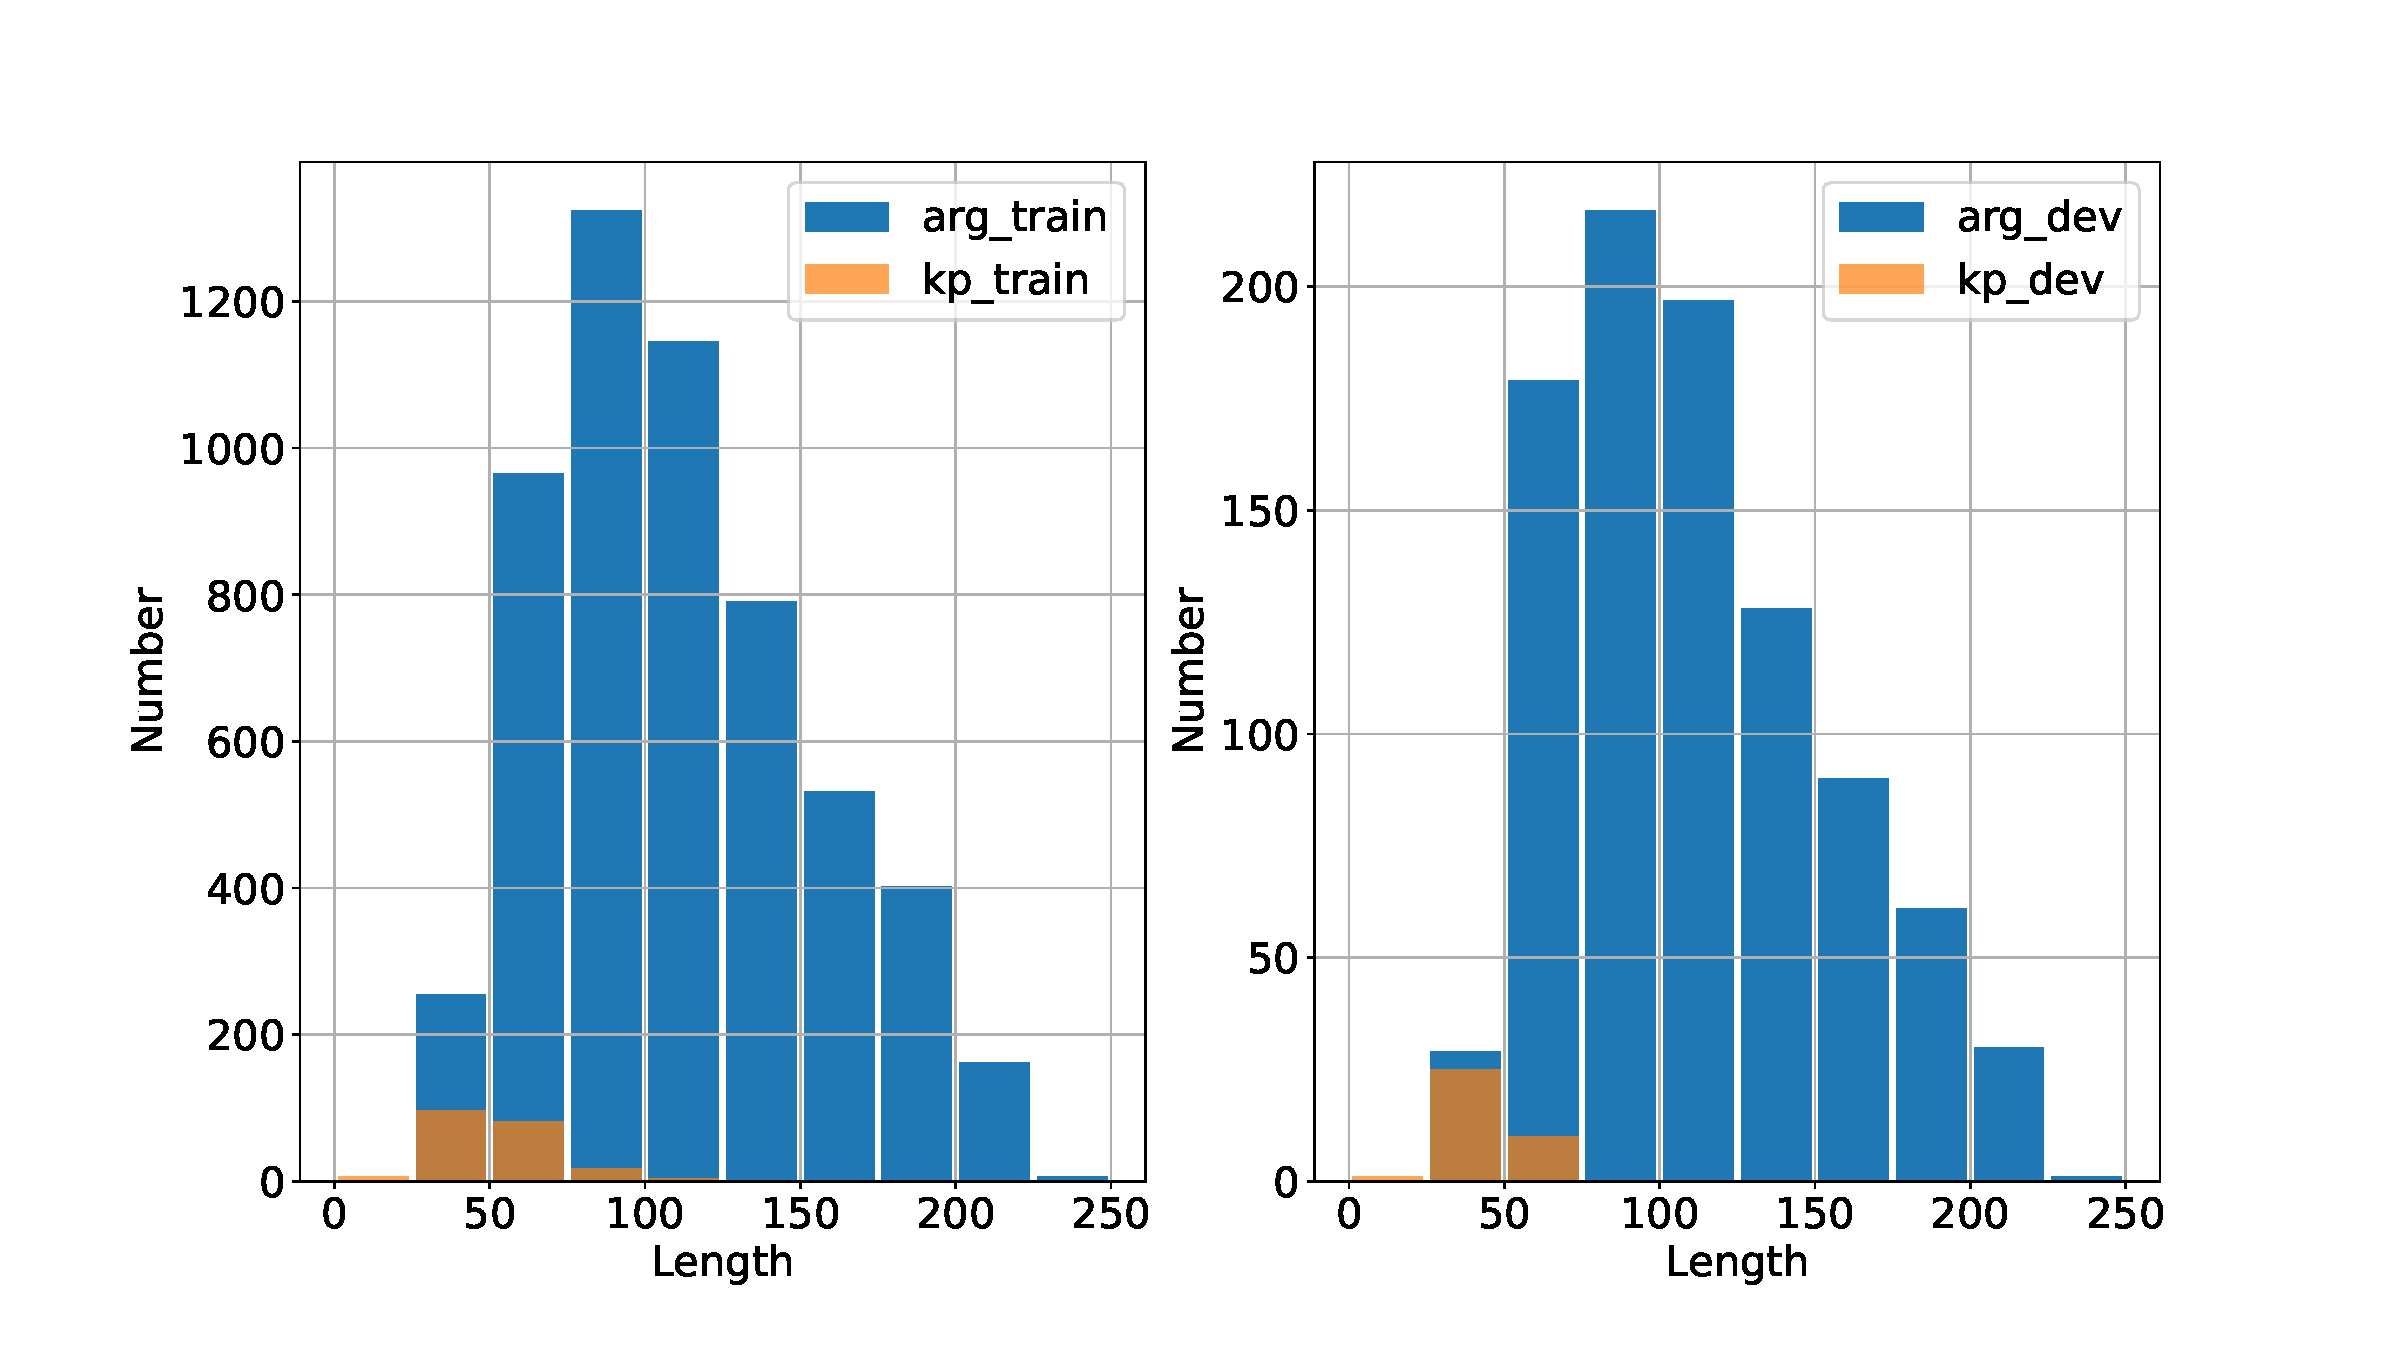
\includegraphics[width=\linewidth]{arg-kp-length.pdf}
    \label{arg-kp-length}
    \caption{Differences in argument and key point lengths in the training and development set.}
\end{figure*}

Furthermore, the arguments in both datasets, the training set, and the validation set, are longer than the key points \todo{see figure}. 
The average length of the arguments is about 109 tokens and of the key points is about 51.7 tokens. 
An argument can be supported by several key points. This set of all matching key points can be called the summary of the given argument.  
In the validation dataset, the key points have an average length of 41.3 tokens, less than in the training dataset, while the average length of the arguments remains almost the same at 107 tokens. 
We also have the average length of a token from the training dataset of 7.5 characters and from the validation dataset of 7 characters. 
The differences in length between arguments and key points from the training dataset and validation dataset are 57.8 and 66.3 respectively. 
This means that the arguments from the training data set are on average about 7.6 tokens longer than the key points and the validation data set is about 9.5 tokens longer. 
From this, we can interpret that the long arguments in the validation set are summarised stronger than the arguments from the training set. 
The proportion of arguments that are more than 66.3 letters longer than key points is about 39\% of the training set and about 44\% of the validation set. We can see that there are more long arguments in the validation set. 
We analyze the effect of this characteristic on the classification model further by results and error analysis (Section \ref{error-analysis}).
